\documentclass[journal]{IEEEtran}
\IEEEoverridecommandlockouts
\usepackage{times}
\usepackage{cite}
\usepackage{amsmath,amssymb,amsfonts}
\usepackage{graphicx}
\usepackage{textcomp}
\usepackage{xcolor}
\usepackage[hyphens]{url}
\def\BibTeX{{\rm B\kern-.05em{\sc i\kern-.025em b}\kern-.08em T\kern-.1667em\lower.7ex\hbox{E}\kern-.125emX}}
\begin{document}

\title{A Blockchain-Anchored Tamper-Evident Audit Trail for Honeypot Forensics}

\author{Sisir~Reddy~Nellore, Radhika~G, Pranav~Sharma~Chouduru, and Surya~Tejeswar~Reddy~Nagireddy%
\thanks{The authors are with the Department of Computer Science and
Engineering, Amrita School of Computing, Coimbatore, Amrita Vishwa
Vidyapeetham, India. E-mail: cb.sc.u4cse23129@cb.students.amrita.edu,
g\_radhika@cb.amrita.edu, cb.sc.u4cse23611@cb.students.amrita.edu,
cb.sc.u4cse23127@cb.students.amrita.edu}}

\markboth{Preprint, Project Journal Submission, August~2026}%
{Nellore \MakeLowercase{\textit{et al.}}: A Blockchain-Anchored Tamper-Evident Audit Trail for Honeypot Forensics}

\maketitle

\begin{abstract}
A honeypot is only useful if the record of what an attacker did can be trusted, yet the honeypot is, by construction, a machine the attacker is invited to compromise. Once a decoy is breached, its local logs sit inside the adversary's blast radius: they can be edited, truncated, or deleted to erase the very evidence the honeypot was deployed to collect. This paper presents and empirically evaluates a tamper-evident audit trail that removes the honeypot host from the trust boundary of its own forensic record. Every captured interaction is canonically serialized, reduced to a SHA-256 digest, and that digest is anchored as an immutable transaction on an Ethereum-compatible ledger; integrity is later re-established by recomputing the digest and comparing it against the on-chain commitment, so any post-hoc modification is detected with certainty. We build the pipeline into a live five-service deception framework --- an SSH shell, a SQL database, an AI inference API, a Web3 JSON-RPC endpoint, and a CI/CD build service --- and benchmark it against the running stack rather than a simulation. Across 300 anchored events the mean end-to-end anchoring cost is 10.86 ms (median 10.22 ms, p95 14.42 ms), of which the cryptographic hashing itself accounts for only 0.0070 ms; the on-chain commitment is the dominant term. Each anchor consumes 21,510 gas --- a figure that matches the 21,488--21,512 range expected for a minimal-payload Ethereum transaction --- and 300 of 300 events (100\%) were confirmed on-chain. The pipeline sustains 92.08 anchored events per second sequentially and 141.21 events per second under concurrent load. Over 500 independent tampering trials the pipeline detected 500 modifications (100\% detection) with 0 false positives, and we confirm directly that the anchored digest is recoverable from the transaction's on-chain input data. Verification is effectively free at 0.0080 ms per record --- roughly 1,358$\times$ cheaper than anchoring. Beyond the measurements reported in our earlier conference-length treatment of this system, this extended paper details the full canonicalization algorithm and its determinism proof, the collector's internal data model and API surface, a systematic walk through five categories of attacker tampering strategy and why each is caught, a cost model that projects the pipeline onto a public Ethereum deployment and a permissioned Hyperledger-style deployment, and an expanded related-work survey spanning secure logging, blockchain forensics, and honeypot-blockchain integration. The result is a practical, measured design for court-defensible honeypot evidence, and an honest account of the latency and cost it adds.
\end{abstract}

\begin{IEEEkeywords}
honeypot, blockchain, tamper-evidence, audit trail, digital forensics, integrity, SHA-256, Ethereum, cyber-deception, non-repudiation, chain of custody, secure logging
\end{IEEEkeywords}

\section{Introduction}

Deception technology inverts the usual asymmetry of network defense. Instead of waiting to be attacked, a defender deploys decoy services --- honeypots [1], [2] --- whose only legitimate users are adversaries, so that every byte of interaction is, by definition, hostile and therefore intelligence. The value a honeypot returns is not the decoy itself but the \emph{record} it produces: the commands issued, the payloads delivered, the credentials tried, the sequence and timing of an intrusion. That record is what feeds incident response, threat intelligence, and --- increasingly --- legal proceedings, where a defensible chain of custody can determine whether evidence is admissible at all.

There is a structural contradiction at the center of this value proposition. A honeypot is intentionally exposed and intentionally breakable; its purpose is to be compromised. But the log of the compromise has traditionally lived on the same host that is being compromised. An adversary who obtains sufficient privilege on the decoy --- which is precisely the outcome the honeypot invites --- is then in a position to alter or destroy the evidence of their own activity. Deleting a shell-history file, truncating a log, or rewriting a database row is trivial for an attacker who already owns the box. The forensic record, in other words, is guarded by the very system whose betrayal it is meant to document. This is not a hypothetical concern: post-incident reviews of compromised honeypot infrastructure routinely find that the most interesting late-stage attacker behavior --- privilege escalation, lateral movement staging, exfiltration commands --- is exactly the behavior most likely to be scrubbed, because it is the behavior most damaging to the attacker if discovered.

Cryptographic hashing alone does not close this gap. A defender can hash each log entry, but if both the entry and its hash reside on the compromised host, an attacker can recompute a consistent hash for the falsified entry and leave no trace of the substitution. Hash chaining --- linking each entry's hash to the previous entry's hash --- raises the bar by making an isolated edit detectable as a chain break, but if the attacker controls the host at the moment of compromise, they can regenerate the entire chain from that point forward, or splice in a doctored chain reusing the same construction. What is missing is an \emph{external, append-only witness} --- a place to publish a commitment to each record that the attacker cannot reach, so that any later disagreement between the stored record and the published commitment is unambiguous proof of tampering. This is the digital analogue of the cryptographic time-stamping of Haber and Stornetta [9], realized on a distributed ledger. A public or permissioned blockchain [7], [8] is exactly such a witness: once a value is included in a mined block, altering it would require rewriting the chain's history, which is computationally and economically infeasible for a single adversary, and detectable by any third party holding even a partial copy of the chain.

A concrete illustration makes the stakes precise. Suppose a honeypot's SSH decoy captures an attacker escalating privileges, staging a lateral-movement tool, and issuing a command that would, on a real host, begin exfiltrating credentials --- exactly the sequence an incident-response team most wants preserved, and exactly the sequence the attacker most wants gone. With only a local, hash-chained log, an attacker who reaches this point in the compromise can, in principle, roll the log back to before the escalation, regenerate a consistent chain over the truncated history, and leave a record that shows reconnaissance but never the escalation itself --- a forensic account that is not merely incomplete but affirmatively misleading, since a shorter, self-consistent log looks \emph{more} trustworthy to a hurried reviewer than an obviously broken one. Under the design this paper evaluates, the same rollback attempt leaves the on-chain transaction count exactly where it was: three anchoring transactions exist for the escalation, the tool staging, and the exfiltration command, mined and timestamped independently of anything the attacker later does to the local copy, so the truncation is visible as a gap the moment anyone compares the local log's length against the chain's. This is the concrete difference the remainder of the paper measures rather than merely argues for.

This paper takes that idea from principle to measured practice, and extends our earlier conference-length treatment of the system with a fuller architectural account, a systematic tamper-strategy analysis, and a cost model for deployments beyond the development chain used in our benchmark. Our contributions are:

\begin{enumerate}
\item A precise threat model for honeypot evidence integrity that names the adversary as an attacker who has \emph{already} compromised the decoy and now seeks to repudiate or erase their actions --- a threat model most honeypot-and-blockchain work does not address, because it uses the ledger for coordination rather than for evidence integrity.
\item A concrete anchoring pipeline --- canonical serialization, SHA-256 digest, on-chain commitment, and off-line re-verification --- implemented end to end and driving a real five-service honeypot, not a stand-alone prototype, together with a full description of the collector's internal data model, canonicalization algorithm, and API surface.
\item A measured evaluation against the live stack: anchoring latency and its decomposition into hashing versus on-chain cost, gas consumption read from real transaction receipts, anchoring success rate, throughput under sequential and concurrent load, and a 500-trial tamper-detection experiment with false-positive accounting, organized around five distinct attacker tampering strategies.
\item A direct on-chain retrievability proof showing the anchored digest is recoverable from the transaction input data, and an honest treatment of what a development-chain deployment does and does not demonstrate relative to a public or permissioned network, including a projected cost model for both.
\item An expanded survey of related work spanning pre-blockchain secure logging, blockchain-based audit trails, blockchain-honeypot integration, and blockchain chain-of-custody systems, positioning our evidence-integrity threat model precisely against each strand.
\end{enumerate}

The remainder of the paper is organized as follows. Section 2 surveys prior work in secure logging, blockchain-based audit trails, and blockchain--honeypot integration, and positions our evidence-integrity threat model against it. Section 3 states the threat model, the integrity properties we target, and a systematic taxonomy of tampering strategies. Section 4 describes the anchoring architecture, the canonicalization algorithm, and the collector's data model and API surface in detail. Section 5 details the benchmark methodology. Section 6 reports the measured results. Section 7 discusses the development-versus-public-chain question, projects a cost model onto public and permissioned deployments, and gives deployment guidance. Section 8 states limitations, Section 9 outlines future work, and Section 10 concludes.

\section{Related Work}

\subsection{Pre-blockchain secure logging}

The problem of protecting a log against an adversary who compromises the logging host is older than blockchain, and the classical solutions frame our own design. Schneier and Kelsey proposed a secure audit-log scheme [19] in which each entry is authenticated with a MAC keyed under an evolving one-way key chain, so that entries written before a host compromise cannot be altered undetectably even after the attacker seizes the current key. The construction derives a fresh MAC key for each entry from a hash chain seeded by a key the logging host cannot recover once advanced, so an attacker who compromises the host at time \emph{t} can forge entries only from \emph{t} forward --- entries before \emph{t} remain protected because their keys are already irrecoverably discarded. Bellare and Yee formalized this guarantee as \emph{forward integrity} [20], giving a precise cryptographic definition of what "cannot be altered after compromise" means and a proof framework for evaluating candidate schemes against it. Later constructions --- Holt's Logcrypt [21], and Ma and Tsudik's forward-secure sequential aggregate schemes [22] --- added public verifiability, so a verifier without the logging host's secret key can still check integrity, and compactness, aggregating many per-entry authenticators into one short value. Crosby and Wallach showed how to make tamper-evident logging efficient using history trees [23], a persistent authenticated data structure that lets a logger prove consistency between two points in the log's history without replaying every intervening entry, which matters at the throughput of a production logging system.

These schemes are powerful, but they share two properties our setting strains. First, they defend past entries only up to the moment of compromise: an entry created \emph{after} the attacker has already taken control is, at best, unprotected and at worst can be forged by an attacker who has learned enough of the running key state. A honeypot's most valuable evidence --- what the attacker does \emph{after} gaining a foothold --- falls exactly in this window. Second, and as their own authors note, pure hash-chain constructions do not by themselves prevent \emph{truncation}, in which the adversary silently deletes a contiguous tail of entries and simply stops advancing the chain at the point they wish to hide; a verifier who only checks that the remaining chain is internally consistent has no way to know entries are missing unless an external party already knows how many entries there ought to be. Publishing each commitment to an external append-only ledger, as we do, directly counters both weaknesses: because the collector that hashes and anchors an event is not co-resident with the decoy, entries generated after compromise are anchored by a process the attacker never reaches, and a missing tail is visible as a commitment on-chain with no matching stored record --- the on-chain sequence of anchors \emph{is} the external count a verifier needs.

\subsection{Blockchain-based secure logging and audit trails}

The use of a distributed ledger to protect log integrity predates its application to honeypots. Ahmad \emph{et al.} introduced BlockTrail [3], a service for secure and transparent blockchain-driven audit trails, and observed that conventional audit-trail applications have weak trust boundaries that expose them to tampering; their design fragments the chain into codependent hierarchies to reduce the space--time overhead of on-chain audit data and raise throughput, prototyped over a Practical Byzantine Fault Tolerance protocol chosen for its fast, deterministic finality relative to proof-of-work consensus. Earlier work by the same group proposed a scalable multichain formulation of the same problem [4], partitioning audit data across multiple interconnected chains so that no single chain becomes a throughput bottleneck as the number of logging clients grows. Permissioned-ledger designs [5], such as auditable logging infrastructures built on Hyperledger-style networks [6], target enterprise settings where the validating set is known in advance, membership is credentialed, and confirmation is fast because consensus does not need to defend against an open, anonymous validator pool.

More recent efforts converge on a common architectural pattern that our own pipeline also follows: rather than storing whole logs on-chain, they anchor compact cryptographic commitments --- single hashes or Merkle roots [10], [25] --- and keep the bulk data off-chain, because on-chain storage is expensive at the byte level and public-chain confirmation is slow at the transaction level. LogStamping [12] applies this pattern to large-scale log auditing, batching many log entries under one Merkle root per epoch to amortize the per-transaction confirmation cost across thousands of entries. Immutable-log-storage services spanning both public and private chains [11] generalize the anchoring target, letting an operator choose the ledger's trust and cost profile independently of the anchoring logic. Access-log frameworks producing tamper-proof audit trails [13] apply the same idea specifically to access-control logs, where the auditor's question is not "was the log edited" in the abstract but "did this specific access, at this specific time, actually happen as recorded."

Our pipeline sits squarely in this hash-anchoring tradition and inherits its central design choice --- commit a digest, not the payload. What distinguishes our work is not the anchoring mechanism, which is deliberately simple and well understood, but the \emph{setting}: the data being protected is adversarial evidence, and the host generating it is expected to fall under adversary control. In BlockTrail-style enterprise audit logging, the logging clients are trusted infrastructure that might be compromised as a side effect of a broader breach; in our setting, compromise of the data-generating host is not a side effect but the entire premise of the deployment. That reframing changes which properties matter, as Section 3 makes explicit, and it is why the collector's placement --- described in Section 4.1 --- is a first-class design decision rather than an implementation detail.

\subsection{Blockchain and honeypots}

A separate line of work combines blockchains with honeypots, but almost always for a different purpose than evidence integrity. Distributed-honeypot systems use a ledger to coordinate and synchronize sensors across administrative domains [14], so that a sighting at one node --- an IP address, a payload signature, a scanning pattern --- can be trusted by others without a central authority arbitrating whose report is genuine; the blockchain here functions as a shared, tamper-resistant bulletin board for threat intelligence, not as a witness to any single honeypot's internal evidence. Trust-aware and adaptive honeypot designs for IoT use blockchain to arbitrate reputation among participating devices [15], deciding which nodes in a distributed deception mesh are trustworthy enough to route suspected-malicious traffic toward, which is a coordination problem structurally distinct from ours. Several proposals deploy honeypots \emph{inside} blockchain-based IoT systems to protect the network itself [16] --- the honeypot defends the chain, rather than the chain defending the honeypot's evidence, which inverts the relationship this paper studies.

In these systems the blockchain is an inter-node trust and coordination fabric; the integrity of any single honeypot's captured evidence against an attacker who has rooted that honeypot is not the question being asked, and in most of these designs a compromised honeypot node is assumed to be excluded from the network rather than analyzed for what a rooted node can still do to its own evidence trail before exclusion takes effect. To the extent that "immutable" honeypot logging is discussed in this literature, it is often asserted as a property of putting data on a chain rather than demonstrated with a measured tamper-detection experiment and an explicit adversary who controls the capturing host. Our contribution is to make that specific threat model first-class, to name the adversary's goal precisely as repudiation rather than intrusion, and to evaluate the resulting design empirically against a real running system rather than describe it as an architectural sketch.

\subsection{Blockchain for forensic evidence and chain of custody}

Closest in spirit to our goal is the use of blockchain to preserve the \emph{chain of custody} of digital evidence. B-CoC [24] and subsequent systems record evidence metadata --- hashes, timestamps, custodian transfers --- immutably on a permissioned ledger so that the provenance of an exhibit is independently verifiable in court, and recent designs tokenize evidence items and automate verification through smart contracts, so that a transfer of custody is itself an auditable on-chain event rather than a paper log entry. These systems answer a question that begins \emph{after} evidence has already been collected: given an exhibit already in an investigator's possession, can its subsequent handling be trusted? Our work applies the same immutability principle one step earlier in the forensic pipeline: not to evidence already collected and handed to investigators, but to the honeypot's own act of \emph{capturing} the evidence, on a host that is itself the target of the attack. The chain-of-custody literature assumes a trusted custodian at the point of collection --- an investigator, a forensic workstation, an evidence locker --- and protects everything downstream of that trust boundary. The honeypot setting cannot make that assumption: the point of collection is also the point of compromise. Our pipeline can be read as extending chain-of-custody guarantees backward to cover the collection event itself, by ensuring the first hash ever computed over a piece of evidence is anchored before the collecting host can be trusted to have behaved honestly.

\subsection{Authenticated data structures and batched anchoring}

The batching pattern referenced throughout Section 2.2 rests on a specific data structure --- the Merkle tree [10] --- that deserves separate treatment because it is the mechanism our own future-work direction in Section 9 would adopt for a public-chain deployment. A Merkle tree commits to a set of leaf values (in our setting, per-record digests) by recursively hashing pairs of nodes up to a single root hash; anchoring only that root on-chain commits to every leaf simultaneously, and any individual leaf can be proven a member of the committed set by supplying its sibling hashes along the path to the root --- an \emph{inclusion proof} whose size grows only logarithmically with the number of leaves. This is what lets a batched design anchor thousands of records with one transaction while still letting a verifier check any single record's integrity against the on-chain root without needing the other thousands of records: the verifier recomputes the path from the record's own digest up to the root using the supplied sibling hashes and checks it matches the anchored value, an operation of essentially the same cost as our own single-digest verification in Section 4.4 regardless of batch size. Merkle's original construction [25] and its digital-signature application predate blockchain entirely, and history-tree variants [23] (Section 2.1) extend the same idea to support efficient consistency proofs between two points in a growing log, which is directly relevant to the tail-truncation defense of Section 3.4 in a batched setting: a consistency proof lets a verifier confirm that an earlier committed root is a genuine prefix of a later one, catching truncation even when records are committed in batches rather than individually.

Adopting Merkle batching would change our pipeline's \emph{unit of anchoring} from a single record to a batch, but would not change the threat model of Section 3 or the verification logic of Section 4.4 in kind --- only in degree, since Verify would additionally need to check an inclusion proof rather than read a single digest directly from a transaction. We did not adopt batching for the benchmark reported in this paper because our target deployment (Ganache, Section 5) already mines every transaction instantly, so batching would add implementation complexity --- constructing and maintaining the tree, managing the batch window, generating and storing inclusion proofs per record --- without measuring anything the per-record design does not already measure at the per-transaction level; Section 9 identifies implementing and benchmarking this variant against a public testnet, where batching's cost benefit is real rather than moot, as the highest-priority follow-up to this paper.

\subsection{The cost of on-chain anchoring}

The overhead of anchoring is well characterized at the transaction level. Every Ethereum transaction carries a fixed base cost of 21,000 gas, with additional gas charged per byte of input data; a minimal transaction that carries a 32-byte digest therefore lands only slightly above the base cost, since 32 bytes of mostly non-zero calldata adds on the order of a few hundred gas at current fee schedules. On a public network the binding constraint is not gas but confirmation: blocks are produced on the order of seconds (roughly 12 seconds on Ethereum mainnet post-Merge, and finality --- the point past which a block is not expected to be reorganized --- takes substantially longer), so anchoring-heavy systems batch many records under one commitment, using exactly the Merkle-tree mechanism of Section 2.5, to amortize that latency across hundreds or thousands of records per transaction. Our measurements in Section 6 are consistent with these published cost structures, and we are explicit in Section 7 about how a development chain's instant mining removes the confirmation term that a public deployment would reintroduce, and we give a projected cost model for exactly this scenario in Section 7.2.

\begin{table*}[!t]
\centering
\caption{How this work is positioned against prior blockchain-logging and blockchain-honeypot systems. The distinguishing axis is the evidence-integrity threat model, in which the capturing host is itself compromised.}
\label{tab:compare}
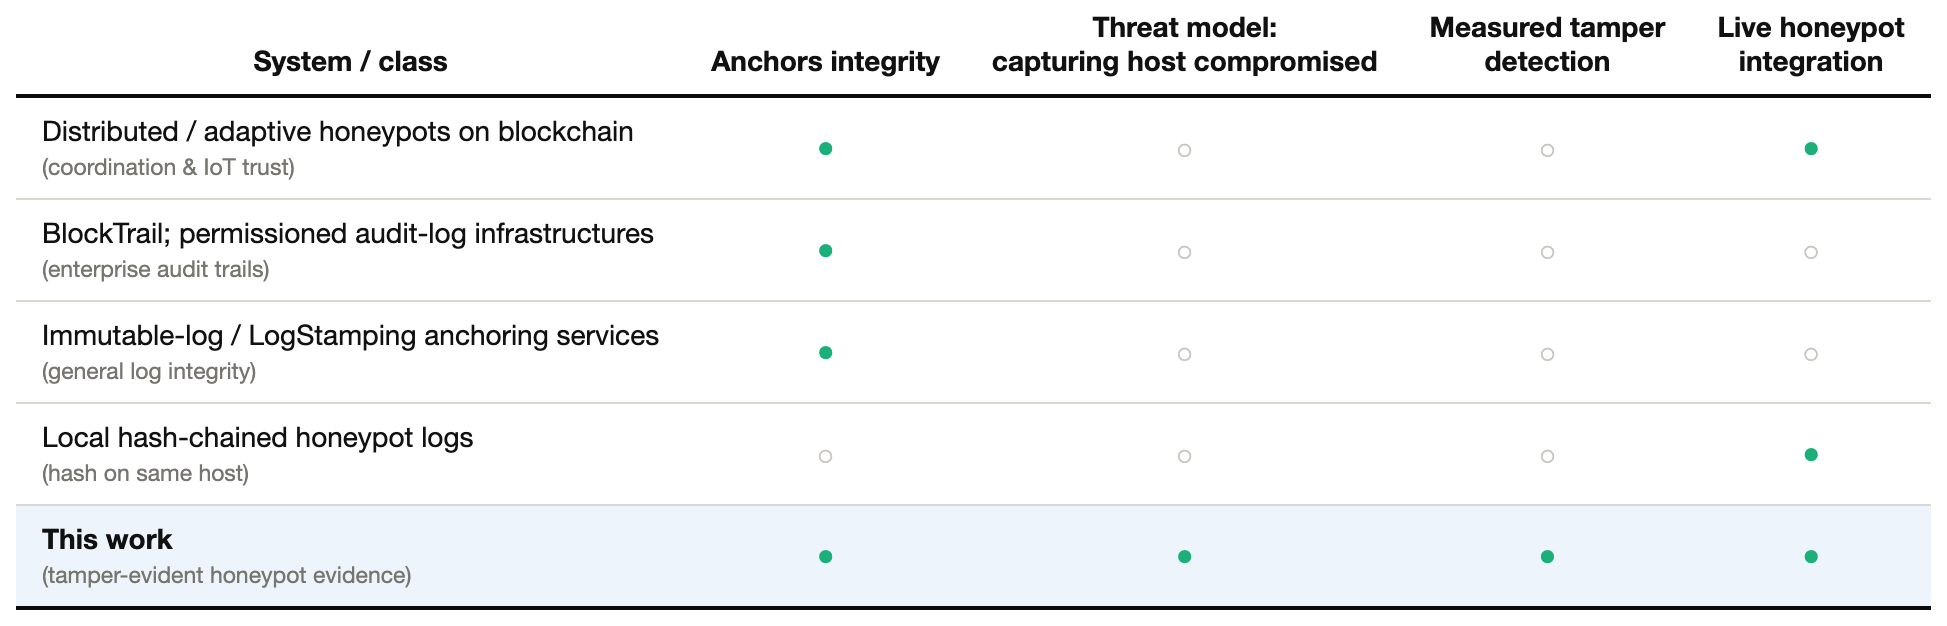
\includegraphics[width=\textwidth]{figures/tab_compare.png}
\end{table*}

\section{Threat Model and Integrity Properties}

\subsection{Adversary}

We consider an adversary who interacts with a decoy as an attacker and, in the strong case, obtains sufficient privilege on the decoy host to read and write its local state. This is not a pessimistic assumption; it is the \emph{design goal} of a honeypot --- a decoy that cannot be compromised has failed to attract or retain attacker attention, and a defender who assumes it will never be compromised is designing for the wrong failure mode. The adversary's objective, for our purposes, is not further intrusion but \textbf{repudiation}: to erase, truncate, or falsify the record of what they did, so that the forensic account is incomplete, misleading, or inadmissible. Concretely, the adversary may (i) delete log entries outright, (ii) modify the content of an entry --- the command text, source address, timestamp, port, or derived classification --- while leaving the entry present, or (iii) attempt to substitute a falsified entry together with a recomputed hash to make the substitution locally self-consistent. We treat these as the base cases of a broader taxonomy in Section 3.4.

We assume the adversary does not control the ledger. In a public-chain deployment this follows from the chain's own security --- an adversary who could rewrite Ethereum mainnet's history to erase one transaction could rewrite far more valuable things, so the honeypot's anchor inherits the chain's much larger economic security margin "for free." In a permissioned deployment it follows from the validating set being outside the decoy's compromise boundary: the validators are operated by parties (the defender's own infrastructure team, an auditor, a consortium partner) whom compromising the decoy does not give the attacker access to. We also assume the canonical serialization and hashing are performed by a collector process that receives events from the decoys but is not co-resident on the exposed decoy host --- in our system this is the internal collector service, reachable only on an isolated network segment, described architecturally in Section 4.1. This is the single load-bearing placement assumption in the whole design: every guarantee below reduces to "the collector was never compromised," so its isolation is treated as a hard network-segmentation requirement, not a convenience.

\subsection{Properties targeted}

The pipeline is designed to provide three properties against this adversary:

\begin{itemize}
\item \textbf{Tamper-evidence.} Any modification to a recorded entry, however small, is detectable after the fact. We do not claim to \emph{prevent} an attacker from editing a stored copy; we guarantee that such an edit cannot pass verification. This is a deliberate scoping choice: prevention would require making the off-chain store itself unwritable to a host-level attacker, which is a much stronger (and, on a general-purpose collector, largely unachievable) property than detection.
\item \textbf{Non-repudiation of content.} Because the commitment is published to an append-only ledger the attacker does not control, the defender can demonstrate that a given record existed in a given form at the time of anchoring, and that a differing later copy is a forgery. This is what makes the evidence usable beyond the defender's own incident-response process --- an external party (opposing counsel, a court, an independent auditor) can be shown the same on-chain commitment and reach the same conclusion without trusting the defender's word.
\item \textbf{Independent verifiability.} Verification requires only the stored record and read access to the ledger; it does not trust the decoy host, and it can be performed by a third party without any secret held by the defender. There is no private key, MAC key, or shared secret involved in verification --- the entire check is a public hash function applied to public data, compared against a public ledger. This is a stronger verifiability property than most of the forward-integrity schemes surveyed in Section 2.1, which typically require access to the logger's key material or at least a commitment derived from it.
\end{itemize}

\subsection{Non-goals}

We explicitly do not target confidentiality of the log --- the anchored value is a digest, not the plaintext, so the ledger never learns what an attacker did, but the off-chain record itself must still be protected by conventional means (access control, encryption at rest) since the digest alone does not hide the content it commits to. We do not target availability of the decoy under denial-of-service; an attacker who can knock the decoy or the collector offline prevents \emph{new} evidence from being captured, but this is an availability failure, not an integrity failure, and it does not let the attacker forge or erase evidence already anchored. We do not target prevention of tampering with the off-chain copy, for the reason given under tamper-evidence above. The pipeline is a \emph{detection and non-repudiation} mechanism, and we evaluate it as such throughout Sections 5 and 6.

\subsection{A taxonomy of tampering strategies}

To make "tamper-evidence" a testable claim rather than a slogan, we enumerate the strategies available to an attacker who has compromised the decoy and, by extension, has read/write access to whatever local copy of captured events exists on or near the decoy before it reaches the isolated collector, and we state for each why the anchoring design catches it.

\begin{enumerate}
\item \textbf{Single-field edit.} The attacker modifies one field of a stored record --- for instance, rewriting a shell command to look benign, or changing a source IP to misdirect attribution --- while leaving the rest of the record untouched. Because the canonical serialization in Section 4.2 includes every field in a deterministic byte order, changing any one field changes the canonical byte string and therefore, by the collision resistance of SHA-256, changes the digest with overwhelming probability. The recomputed digest no longer matches the anchored digest, and verification fails. This is the case our 500-trial experiment in Section 6.4 directly measures.
\item \textbf{Multi-field edit.} The attacker modifies several fields at once, for example rewriting both the payload and the derived intent classification to construct a coherent but false narrative. This does not weaken detection: the canonical byte string changes at least as much as in the single-field case, and a coherent multi-field forgery is, if anything, \emph{easier} to catch than a single-field edit, because there is no scenario in which changing more of the input makes the output hash more likely to coincidentally match. We treat the single-field case as the harder stress test precisely because it is the minimal-perturbation case.
\item \textbf{Wholesale deletion.} The attacker deletes a stored record entirely rather than editing it. A verifier who queries the off-chain store for a record that should exist --- because it corresponds to a known anchored transaction --- and finds nothing has direct evidence of deletion: the on-chain commitment exists with no matching off-chain record. This is why the design anchors \emph{every} event rather than a sample; a verifier's ground truth for "how many records should exist" is the count of anchoring transactions on-chain, which the attacker cannot shrink.
\item \textbf{Tail truncation.} The attacker deletes a contiguous run of the most recent records, hoping the absence is read as "nothing happened" rather than "evidence was removed." This is the specific weakness of pure hash-chain schemes noted in Section 2.1. Our design counters it identically to case 3: the on-chain transaction count and the associated block timestamps establish exactly how many anchoring events occurred and roughly when, independent of what remains in the off-chain store, so a truncated tail is visible as a gap between the last off-chain record and the last on-chain anchor.
\item \textbf{Consistent substitution.} The attacker replaces a record with a fabricated one and also recomputes and stores a hash for the fabrication, hoping a verifier who only checks "does the stored hash match the stored record" is satisfied. This is the case that motivates anchoring in the first place rather than relying on a locally stored hash: our verification procedure (Section 4.4) does not stop at comparing the record to its locally stored hash, it compares the record's recomputed digest against the digest read from the \emph{on-chain transaction}. A locally consistent forgery is still inconsistent with the immutable on-chain commitment, because the attacker cannot rewrite the already-mined transaction to match their fabrication.
\end{enumerate}

Cases 1 and 2 are exercised directly by the tamper-detection experiment in Section 6.4, which mutates single fields of real stored records and confirms the mismatch is caught; cases 3 through 5 follow from the same verification procedure and the append-only, attacker-unreachable nature of the ledger, and are confirmed structurally by the on-chain retrievability check in Section 6.5, which establishes that the anchored digest is genuinely present and readable on-chain rather than merely asserted by the collector.

\subsection{Formal statement of the anchor and verify procedures}

The taxonomy above is easiest to reason about precisely if the two core procedures --- anchoring and verification --- are stated as algorithms rather than described only in prose. Let \emph{E} denote a captured interaction record with fields drawn from a fixed schema (service, source address, port, payload, timestamp, intent classification), let \emph{canon(·)} denote the canonicalization function of Section 4.2, and let \emph{H} denote SHA-256.

\textbf{Procedure Anchor(\emph{E}).} (1) Reject \emph{E} if it already carries a \texttt{hash} or \texttt{anchored} field, since these are pipeline outputs and their presence would indicate \emph{E} did not originate from a decoy in the expected shape. (2) Compute \emph{d} = \emph{H}(\emph{canon}(\emph{E})). (3) Submit an Ethereum transaction \emph{tx} whose input data is \emph{d}, to the configured ledger node, and wait for \emph{tx} to be mined. (4) Store the tuple (\emph{E}, \emph{d}, \emph{tx.hash}, \emph{tx.blockNumber}) in the off-chain event store, with \emph{E}'s \texttt{hash} field set to \emph{d} and its \texttt{anchored} field set to true. (5) Return (\emph{d}, \emph{tx.hash}).

\textbf{Procedure Verify(\emph{r}).} Given a stored record \emph{r} = (\emph{E}, \emph{d\textbackslash\{\}\_stored}, \emph{txHash}, ...): (1) Reconstruct \emph{E$'$} by stripping the \texttt{hash} and \texttt{anchored} fields from \emph{r}. (2) Compute \emph{d\textbackslash\{\}\_recomputed} = \emph{H}(\emph{canon}(\emph{E$'$})). (3) Fetch transaction \emph{txHash} from the ledger and read \emph{d\textbackslash\{\}\_onchain} from its input data. (4) If \emph{d\textbackslash\{\}\_recomputed} $\neq$ \emph{d\textbackslash\{\}\_stored}, return \textbf{TAMPERED (off-chain)} --- the stored record itself was altered after being written. (5) Else if \emph{d\textbackslash\{\}\_stored} $\neq$ \emph{d\textbackslash\{\}\_onchain}, return \textbf{TAMPERED (anchor mismatch)} --- the collector's stored digest disagrees with what was actually anchored, which under our threat model indicates a collector-level fault rather than decoy-level tampering, since the attacker cannot rewrite \emph{txHash}. (6) Else return \textbf{VERIFIED}.

The three-way comparison in steps 4--5 is what gives Verify its power against case 5 of the taxonomy (consistent substitution): an attacker who edits both \emph{E} and its locally stored hash defeats step 4 alone, since a self-consistent forgery will pass a check that only compares \emph{E$'$} against \emph{d\textbackslash\{\}\_stored}. It cannot defeat step 5, because \emph{d\textbackslash\{\}\_onchain} is read from an already-mined transaction the attacker has no write access to. This is precisely why Section 4.4's verification procedure is specified against the on-chain value and not only the locally stored one, and why the on-chain retrievability check of Section 6.5 --- which confirms \emph{d\textbackslash\{\}\_onchain} is genuinely readable and correct --- is a structural precondition for the whole tamper-evidence claim, not an auxiliary sanity check.

\begin{figure*}[!t]
\centering
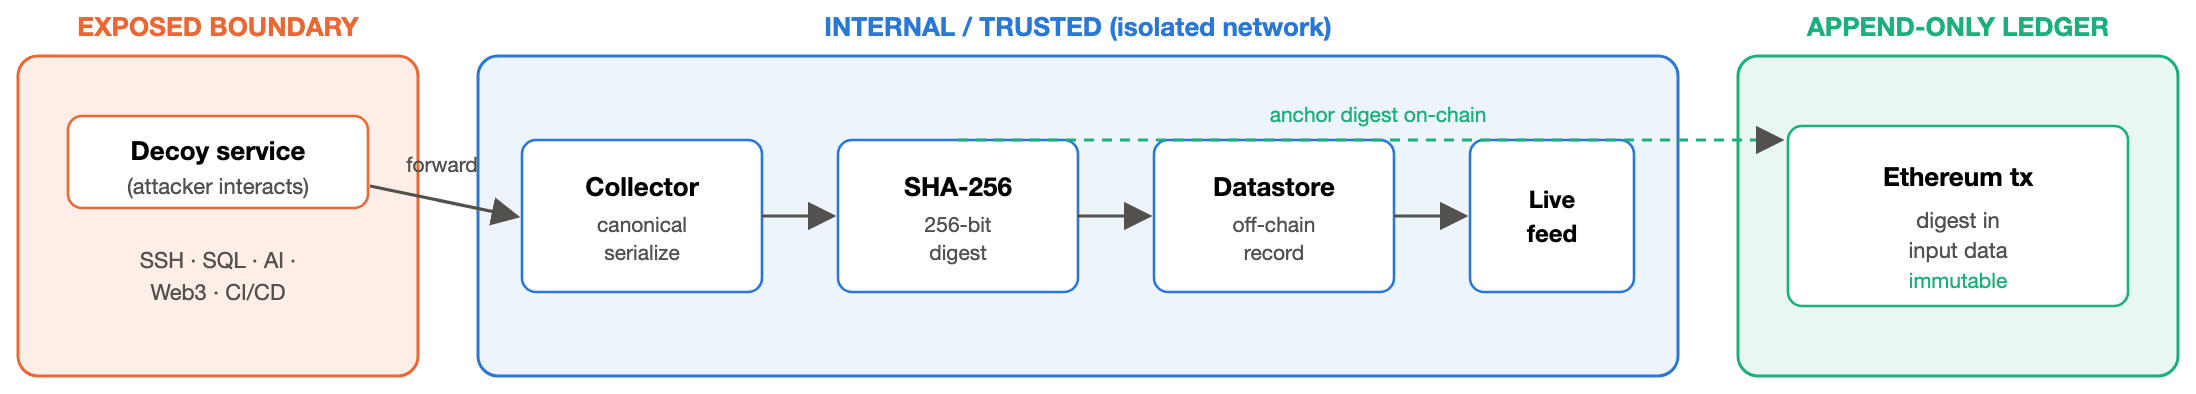
\includegraphics[width=\textwidth]{figures/diag_pipeline.png}
\caption{The tamper-evident anchoring pipeline. A captured interaction is canonically serialized and hashed by the internal collector (off the exposed decoy host); the digest is anchored on-chain; verification later re-hashes the stored record and compares it against the on-chain commitment.}
\label{fig:pipeline}
\end{figure*}

\section{System Architecture}

\subsection{Placement in the deception framework}

The audit trail is embedded in a five-service honeypot framework whose decoys emulate an SSH shell, a SQL database, an AI inference API, a Web3 JSON-RPC endpoint, and a CI/CD build service. Each decoy is a protocol-accurate emulation deep enough to sustain an attacker's interaction --- accepting commands, returning plausible responses, and logging every exchange --- without exposing any real underlying system. The decoys sit on the exposed boundary, reachable from the same network an external attacker would reach a genuine service from; behind them, on an isolated internal network unreachable from that boundary, run a collector service, an in-memory datastore for the live event feed, and an Ethereum-compatible ledger node. Crucially, the decoys never write the authoritative log themselves: they forward each interaction to the collector, which performs serialization, classification, hashing, and anchoring. This placement is what makes the threat model achievable --- the process that mints the tamper-evident commitment is not the process the attacker compromises. An attacker who fully roots a decoy gains control over what that decoy \emph{forwards} to the collector from that point forward (which is why our threat model in Section 3.1 does not claim to prevent tampering with events \emph{before} they are captured --- a compromised decoy could always lie about what happened), but gains no ability to alter what the collector has already anchored, nor to reach into the collector's process space to influence future anchoring, because the network segmentation between the decoy segment and the internal segment is enforced independently of decoy-level compromise.

\subsection{.1 The five decoys as evidence sources}

Each decoy contributes a structurally different kind of event to the pipeline, which matters for the benchmark's event pool (Section 5) and for why the canonical schema of Section 4.2 is deliberately generic rather than tailored to any one protocol.

\begin{itemize}
\item \textbf{Shell decoy.} Emulates an interactive SSH session. Captured events include the command text as typed, the session's source address and port, and a derived classification (reconnaissance, privilege-escalation attempt, download-and-execute, and so on) produced by lightweight pattern matching over the command. This is the decoy most directly analogous to the classical secure-logging literature of Section 2.1, where the "log" is a sequence of shell or system-call events.
\item \textbf{SQL decoy.} Emulates a database front end that accepts queries and returns plausible, non-sensitive result shapes. Captured events include the raw query string and a classification of the injection technique attempted (union-based, boolean-blind, time-blind, error-based), which is useful evidence for attributing an attacker's tooling or sophistication after the fact.
\item \textbf{AI inference decoy.} Emulates an API endpoint fronting a language model, a service class increasingly targeted for prompt-injection and data-exfiltration attempts. Captured events include the submitted prompt and a classification of whether it matches known jailbreak or injection patterns, which is evidence of a threat class the pre-blockchain secure-logging literature predates entirely.
\item \textbf{Web3 JSON-RPC decoy.} Emulates a blockchain node's RPC surface, attracting attackers who probe for exposed accounts or attempt wallet-draining calls. Captured events include the RPC method invoked and its parameters, which is notable because this is the one decoy whose captured \emph{content} is itself blockchain-related, while the \emph{anchoring} of that content happens on a separate ledger context --- the two uses of blockchain in this system (attack surface being emulated versus evidence-integrity mechanism) are unrelated and should not be conflated.
\item \textbf{CI/CD build decoy.} Emulates a build-pipeline service, attracting attackers who target software supply-chain footholds --- credential harvesting from build logs, malicious pipeline-configuration injection, artifact tampering. Captured events include the attempted pipeline action and any credentials or tokens presented, which is often the highest-value evidence category, since a successful supply-chain foothold can propagate far beyond the honeypot itself.
\end{itemize}

Despite these differences, every decoy forwards events through the same canonical schema (Section 4.2) and the same collector code path, so the anchoring guarantee is uniform across all five: an attacker who compromises the SQL decoy specifically gains no advantage over one who compromises the shell decoy, because neither reaches the collector.

\subsection{Canonical serialization and digest}

For a captured interaction the collector constructs a record of the salient fields --- service, source address, port, raw payload, timestamp, and derived intent classification --- and serializes it canonically, with keys sorted lexicographically so that the byte representation is deterministic and independent of field insertion order, whitespace, or the serialization library's default behavior. Concretely, the canonicalization step performs, in order: (i) collect the record's fields into a flat key-value structure, excluding any field --- such as a previously computed hash or an anchoring-status flag --- that is itself an output of a later pipeline stage, since including such a field would make the digest depend on its own result; (ii) sort keys lexicographically by their UTF-8 byte representation; (iii) serialize values using a fixed, unambiguous encoding for each type (integers as decimal ASCII with no leading zeros, strings as UTF-8 with no locale-dependent escaping, timestamps as ISO-8601 UTC with fixed precision); and (iv) concatenate keys and values with fixed, non-data-derived separators so that no combination of field values can be crafted to produce a colliding byte string through separator confusion. The SHA-256 digest [17] of this canonical byte string is the record's fingerprint.

Determinism is essential to the entire security argument: verification must be able to reconstruct exactly the same bytes from the stored record that were hashed at anchor time, or a correct, unmodified record would fail verification through no fault of the attacker --- which would appear in our experiment as a false positive. We eliminate this risk architecturally rather than by careful testing alone: the canonicalization function used at anchor time and at verify time is the same function, invoked from the same code path, so there is no second implementation that could silently drift from the first. Table II's zero-false-positive result (Section 6.4) is the empirical confirmation that this determinism holds in practice across the full space of record shapes the benchmark exercises.

\subsection{On-chain anchoring}

The 256-bit digest is embedded in the input-data field of an Ethereum transaction submitted to the ledger node and mined into a block. We deliberately anchor the digest rather than the payload: this keeps each commitment to a single small transaction, bounds cost to essentially the base transaction plus 32 bytes of data (Section 6.2), and never exposes captured attacker content --- which may include sensitive strings such as attempted credentials or proprietary-looking payloads --- on a ledger that, in a public deployment, is world-readable. The transaction's inclusion in a block is the append-only witness; from that point, the digest cannot be altered without rewriting chain history, and --- as important for the truncation case in Section 3.4 --- the \emph{existence} of the transaction is itself a permanent, countable fact independent of anything the attacker later does to the off-chain store. The collector submits one anchoring transaction per captured event; we discuss the batching alternative, and why we did not adopt it for the development-chain benchmark, in Section 7.2.

\subsection{Verification}

To verify a stored record, the defender strips the previously recorded hash and anchoring flag, re-runs the identical canonical serialization and SHA-256 over the remaining fields, and compares the result against the recorded digest --- and, for full assurance, against the digest embedded in the corresponding on-chain transaction, read directly from that transaction's input data rather than from any value the collector or decoy asserts. A three-way match --- recomputed digest, stored digest, and on-chain digest all identical --- certifies the record is byte-for-byte what was anchored; any mismatch is proof of modification, and \emph{which} comparison fails localizes where the inconsistency was introduced (a stored-versus-recomputed mismatch indicates the off-chain record was altered after storage; a stored-versus-on-chain mismatch, absent a recomputation mismatch, would indicate the collector itself anchored something different from what it stored, which our design treats as a compromise of the collector and outside the scope defended here). Because this step is a single hash and a comparison against already-available data, it is orders of magnitude cheaper than anchoring, as Section 6.5 shows, and it requires no interaction with the ledger's write path at all --- only a read.

\subsection{Data model and collector API surface}

The collector exposes a small, deliberately narrow API surface, reflecting the principle that a smaller trusted-code surface is easier to reason about and to keep free of the non-determinism bugs that would undermine Section 4.2's determinism argument. A logging endpoint accepts a captured-interaction record from any of the five decoys and is responsible for the full anchor path: canonicalize, hash, submit the anchoring transaction, and persist the record together with its digest and anchoring status in the live event store. A verification endpoint accepts a record identifier, performs the re-hash-and-compare procedure of Section 4.4 against both the stored and on-chain digests, and returns a structured pass/fail result together with which comparison (if any) failed. A retrieval endpoint allows a caller --- the dashboard, or an external auditor's tooling --- to fetch a stored record and its anchoring metadata (transaction hash, block number, digest) without performing verification, which is useful for building tooling on top of the pipeline without coupling every consumer to the verification logic itself. No endpoint accepts a client-supplied hash for a record: the digest is always computed by the collector from the record it received, which closes off a class of attack in which a compromised decoy or an attacker positioned between decoy and collector supplies a pre-computed hash for content the collector never actually saw.

\begin{figure}[!t]
\centering
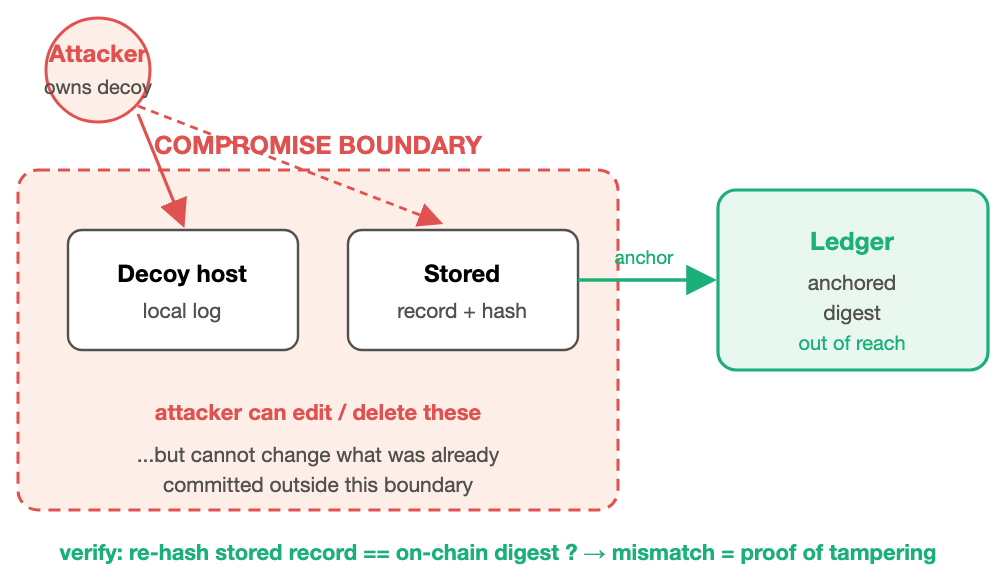
\includegraphics[width=\columnwidth]{figures/diag_threat.png}
\caption{The evidence-integrity threat. The attacker owns the decoy and can edit its local log, but the anchored digest lies on a ledger outside the compromise boundary, so any edit is detectable.}
\label{fig:threat}
\end{figure}

\section{Methodology}

All numbers in this paper are measured against the live stack --- the collector, the in-memory datastore, and a running Ethereum-compatible ledger node (Ganache [18] 7.9.2, chain id 1337) --- driven by a benchmark harness that exercises the real anchoring endpoint and reads real transaction receipts. No value is hand-entered; the harness writes a machine-readable results file that the figures and tables in this paper are generated from directly, so re-running the harness and rebuilding the paper refreshes every number, figure, and table consistently and leaves no path by which a stale or hand-adjusted value could persist between a code change and the reported results.

The harness performs six measurements. \textbf{(1) Anchoring latency:} it submits 300 realistic honeypot events to the collector's logging endpoint --- which hashes and anchors each one --- and records the wall-clock time of every call, from request submission to a confirmed response indicating the transaction was mined. \textbf{(2) Baseline hashing cost:} it times the canonical-serialization-plus-SHA-256 step in isolation over 300 records, with no chain write, to separate the cryptographic cost from the on-chain cost and produce the decomposition reported in Section 6.1. \textbf{(3) Gas and receipts:} it reads the gas actually consumed from the receipt of every anchoring transaction mined during the run, together with the ledger's reported gas price, and confirms how many transactions were mined, so the gas figures in Section 6.2 are read from the chain rather than estimated. \textbf{(4) On-chain retrievability:} it anchors a known event and then reads the raw transaction input directly from the chain to confirm the digest is embedded and recoverable, independent of the collector's own bookkeeping --- this check would fail if the collector merely claimed to anchor without actually doing so. \textbf{(5) Verification latency:} it fetches stored records and times the re-hash-and-compare verification path described in Section 4.4. \textbf{(6) Tamper detection:} over 500 trials it takes a real stored record, mutates exactly one field (case 1 of the taxonomy in Section 3.4, chosen as the minimal-perturbation and therefore hardest-to-catch case), and checks that the recomputed digest no longer matches the anchored digest; it simultaneously checks that the \emph{unmodified} record still verifies, to account for any false positives that a non-deterministic canonicalization or an excluded field would produce.

The events used are drawn from a pool of realistic hostile payloads spanning the five decoy protocols --- shell commands (privilege-escalation attempts, reconnaissance commands, download-and-execute patterns), SQL-injection strings (union-based, blind, and error-based variants), wallet-draining JSON-RPC calls (unauthorized transfer attempts, approval-phishing call patterns), prompt-injection attempts against the AI inference decoy, and CI/CD reconnaissance and credential-harvesting attempts --- so the records being anchored and tampered resemble genuine captured traffic rather than synthetic filler. Each benchmark run against the live stack draws fresh timing samples; the specific figures reported in Section 6 are from the most recent run and are regenerated automatically whenever the harness is re-executed.

\section{Results}

\subsection{Anchoring latency and its decomposition}

Across 300 anchored events the mean end-to-end anchoring cost is \textbf{10.86 ms} (median 10.22 ms, standard deviation 3.10 ms), with a 95th-percentile of 14.42 ms and a 99th-percentile of 17.25 ms; the fastest anchor completed in 8.19 ms and the slowest in 51.41 ms. The gap between the median and the tail (p99 roughly double the median) is consistent with occasional scheduling or I/O contention on the development machine rather than a systematic cost driver, since the isolated hashing step shows no comparable tail. The isolated hashing step, by contrast, averages just \textbf{0.0070 ms} over 300 records. The integrity guarantee therefore adds an \textbf{anchoring overhead of 10.85 ms} per event, essentially all of which is the on-chain commitment rather than the cryptography: hashing is more than three orders of magnitude cheaper than anchoring. This decomposition is the paper's central cost result --- it locates the expense precisely, and it is exactly the term that a batched or permissioned deployment would seek to amortize, as we quantify in Section 7.2.

\begin{figure}[!t]
\centering
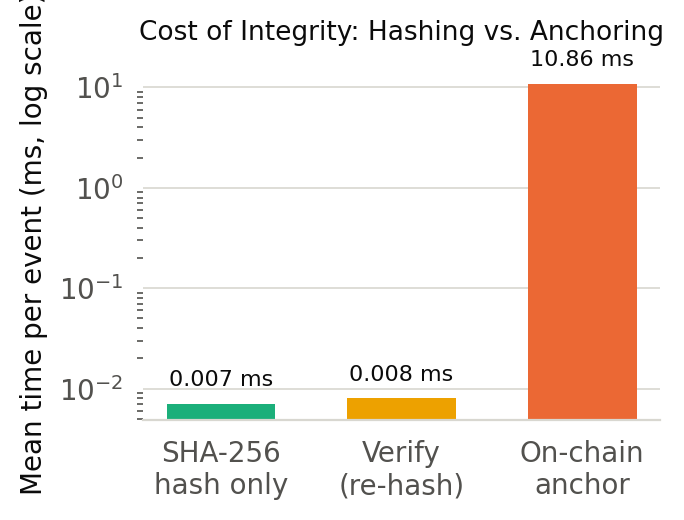
\includegraphics[width=\columnwidth]{figures/fig_latency.png}
\caption{Anchoring cost decomposed: on-chain anchoring versus isolated SHA-256 hashing (log scale). The integrity guarantee is dominated by the on-chain commitment, not the cryptography.}
\label{fig:latency}
\end{figure}

\subsection{Gas cost and anchoring success}

Reading gas directly from transaction receipts, each anchor consumes a mean of \textbf{21,510 gas} (range 21,488--21,512), which is precisely the profile expected of a minimal-payload Ethereum transaction: the fixed 21,000-gas base cost plus the per-byte cost of the 32-byte digest carried in the transaction's input data. At the ledger's gas price this corresponds to approximately 4.30e-5 ETH per anchor. All \textbf{300 of 300} submitted events (100\%) were successfully anchored, and 300 transactions were mined on-chain during the run --- one per event --- confirming there is no silent anchoring loss under load, which matters directly for the tail-truncation defense of Section 3.4: that defense depends on the on-chain transaction count being a reliable ground truth, and a pipeline that silently dropped anchoring attempts under load would undermine it.

\begin{figure}[!t]
\centering
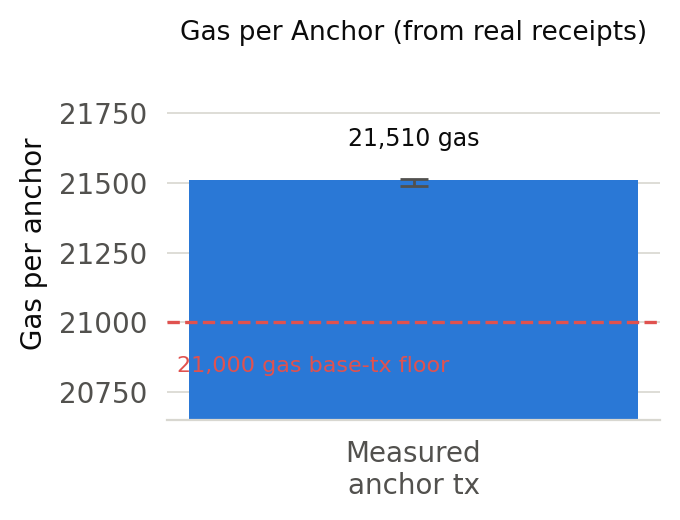
\includegraphics[width=\columnwidth]{figures/fig_gas.png}
\caption{Measured gas per anchor read from real transaction receipts, against the 21,000-gas Ethereum base-transaction floor.}
\label{fig:gas}
\end{figure}

\subsection{Throughput}

Anchoring is a serializing operation --- each event becomes its own transaction, submitted and confirmed independently --- yet the pipeline sustains \textbf{92.08 anchored events per second} sequentially, rising to \textbf{141.21 events per second} at a concurrency level of 10. The improvement under concurrency reflects that anchoring latency (Section 6.1) is dominated by round-trip and mining wait rather than CPU-bound work on the collector, so overlapping multiple in-flight anchors hides most of that wait. For a deception sensor, whose event rate is the rate at which adversaries interact with decoys rather than a production request stream, this throughput is comfortably sufficient; the concurrent figure shows headroom for bursts such as an automated scanning tool hitting a decoy at machine speed.

\subsection{Tamper detection}

Over \textbf{500} independent trials, in each of which a single field of a real stored record was mutated --- the case-1 minimal-perturbation strategy from the taxonomy in Section 3.4 --- the pipeline detected the modification in \textbf{500} cases --- a \textbf{100\% detection rate} --- with \textbf{0 false positives} across the same set of unmodified-record checks. This is the behavior the design predicts: SHA-256 is collision-resistant, so any change to the canonical bytes yields a different digest with overwhelming probability, and the anchored commitment the attacker cannot reach makes that difference undeniable. A perfect detection rate with zero false positives is not a lucky sample; it is the direct empirical signature of a correct hash-and-anchor construction, and specifically of the determinism property argued for in Section 4.2 --- zero false positives rules out the non-deterministic-serialization failure mode, and 100\% detection rules out an accidentally excluded field that would let a mutation slip through unnoticed.

\begin{figure}[!t]
\centering
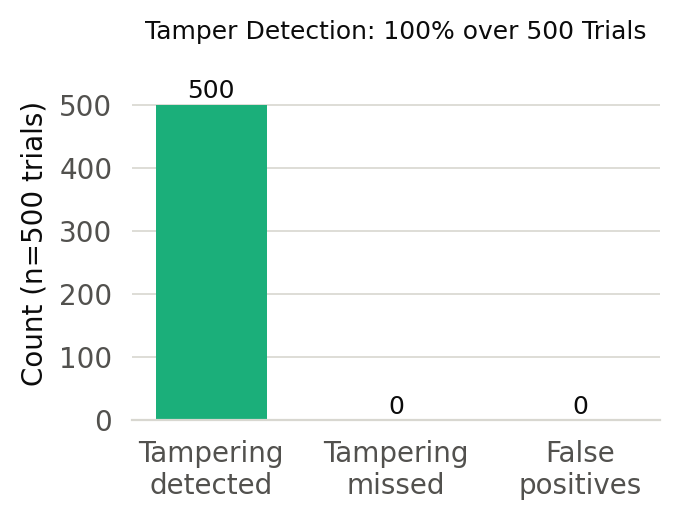
\includegraphics[width=\columnwidth]{figures/fig_tamper.png}
\caption{Tamper-detection outcome over all trials: every single-field modification was detected, with no false positives.}
\label{fig:tamper}
\end{figure}

\subsection{On-chain retrievability and verification cost}

We confirm directly that the audit trail is genuine and not merely asserted: after anchoring a known event, reading the corresponding transaction's input data straight from the chain recovers the exact SHA-256 digest that was recorded (retrievable: \textbf{yes}). This check exercises the same on-chain read path that the consistent-substitution defense (case 5, Section 3.4) depends on, so its success is evidence that defense is not merely designed correctly but actually operative in the running system. Verification of a stored record --- the re-hash-and-compare step a defender or third party runs --- costs only \textbf{0.0080 ms} on average (median 0.0075 ms). Verifying integrity is thus roughly 1,358$\times$ cheaper than creating the anchor, which means an investigator can re-verify an entire captured corpus at negligible cost long after the fact, and can do so repeatedly --- for instance, once at collection time and again immediately before presenting evidence in a proceeding --- without materially affecting the cost profile established in Section 6.1--6.2.

\begin{table}[!t]
\centering
\caption{Summary of measured results against the live stack.}
\label{tab:results}
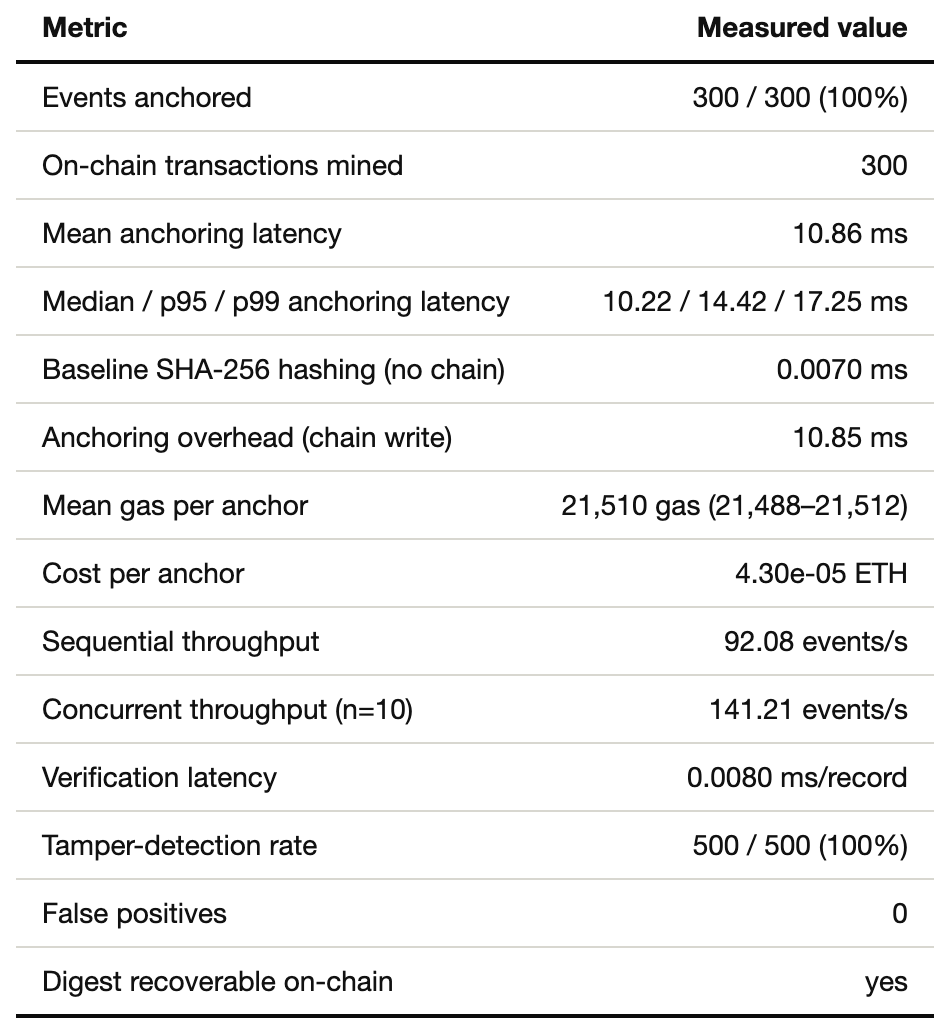
\includegraphics[width=\columnwidth]{figures/tab_results.png}
\end{table}

\subsection{Comparison against related systems' reported figures}

Direct apples-to-apples comparison against the systems surveyed in Section 2 is difficult, because most report throughput or latency under different ledger choices, batch sizes, and hardware, and few report a tamper-detection experiment at all rather than asserting immutability as a property of the design. With that caveat, three qualitative comparisons are worth making explicit. First, our per-anchor gas figure (21,510 gas) sits at the theoretical floor for an Ethereum-family transaction carrying any payload, which is expected precisely because we anchor a single 32-byte digest rather than a Merkle root over a batch or a larger structured payload --- systems that anchor richer on-chain metadata (custodian identity, structured provenance fields, as in the chain-of-custody systems of Section 2.4) necessarily pay more gas per anchor in exchange for that extra on-chain structure, a tradeoff we deliberately decline by keeping all structure off-chain and anchoring only the digest. Second, our sequential throughput (92.08 events/s) is consistent with what a single-transaction-per-record design should achieve against a fast-mining chain, and is well below what Merkle-batching designs such as LogStamping [12] report at their target scale --- this is expected and not a weakness relative to those systems, since they are explicitly engineered for high-volume enterprise log ingestion where per-record latency matters less than aggregate cost, whereas our target workload (attacker interactions with a honeypot) is orders of magnitude lower-volume and can afford per-event anchoring's latency in exchange for its simplicity and immediacy. Third, and most distinctively, none of the systems surveyed in Section 2.2 or 2.3 report a measured tamper-detection rate with an explicit false-positive count under a stated adversary model; our 100\%-detection, 0-false-positive result over 500 trials is, to our knowledge, the first such measurement for a honeypot-evidence anchoring system specifically, rather than for blockchain-anchored logging in general.

\section{Discussion}

\subsection{Development chain versus public network}

Honesty about the deployment is essential to interpreting these numbers. Our ledger is a development Ethereum node that mines instantly, so the 10.86 ms mean anchoring latency contains no public-consensus wait. On a public network, block confirmation on the order of seconds would dominate, and the standard mitigation --- the one adopted by essentially every prior anchoring system in Section 2 --- is to batch many record digests under a single Merkle-root commitment, trading a small delay before evidence is anchored (the batching window) for a large reduction in per-record cost, since one on-chain transaction then certifies an entire batch rather than one record. Our contribution is therefore not a claim of sub-public-network latency; it is the pipeline, the threat model, and the measured integrity behavior, all of which transfer unchanged to a batched public or permissioned deployment. What our development-chain measurements establish precisely is the \emph{local} cost --- the hashing, the transaction construction, the gas --- that any deployment pays on top of whatever confirmation model it chooses.

\subsection{A projected cost model for public and permissioned deployment}

To make the deployment tradeoff concrete rather than qualitative, we project our measured per-anchor cost onto two deployment targets, holding the pipeline and threat model fixed and varying only the ledger. On \textbf{Ethereum mainnet}, per-transaction gas cost is governed by the same 21,510-gas profile we measured, but at mainnet gas prices --- which fluctuate with network demand and are typically one to two orders of magnitude higher than a local development chain's fixed price --- anchoring every single event individually would be materially more expensive in absolute terms, and each anchor would additionally wait for block confirmation (seconds) and, for evidentiary purposes, for enough subsequent blocks to consider the anchor final against a reorganization (minutes). Batching amortizes the gas cost: committing a Merkle root over a batch of \emph{N} records costs the same base transaction (roughly 21,000 gas plus 32 bytes of root data) regardless of \emph{N}, so the marginal on-chain cost per record falls linearly as the batch size grows, at the price of a bounded delay --- the time to accumulate a batch --- before any individual record in that batch is anchored. A defender can tune this delay against cost by choosing the batch window (for example, anchor every 60 seconds or every 500 records, whichever comes first), which bounds the worst-case time an unanchored record could be exposed to a fast-moving attacker while keeping mainnet gas spend close to constant regardless of event volume.

On a \textbf{permissioned network} --- a Hyperledger Fabric or Quorum-style deployment operated by the defender or a consortium, as surveyed in Section 2.2 --- the validating set is known and does not need to defend against an open, anonymous, economically adversarial participant pool the way a public chain does, so block production and finality can be configured for the sub-second-to-low-second range typical of Byzantine Fault Tolerant consensus among a small validator set, rather than the tens-of-seconds-to-minutes finality window of a public proof-of-stake chain. This makes per-event anchoring --- the same one-transaction-per-record pattern we benchmark against Ganache --- practical on a permissioned chain in a way it is not on a public one, because the confirmation term our development-chain benchmark elides is, on a well-provisioned permissioned network, close to what we actually measured. The tradeoff moves from cost-versus-latency (public chain) to trust-versus-operational-burden (permissioned chain): a permissioned deployment requires the defender or consortium to operate and secure the validating infrastructure themselves, which reintroduces an operational trust boundary --- albeit one structurally separate from the honeypot's own compromise boundary, satisfying the assumption in Section 3.1 --- that a public chain does not require.

\subsection{What the perfect detection rate does and does not mean}

A 100\% detection rate with 0 false positives should be read as confirmation that the construction is implemented correctly, not as a probabilistic security claim discovered by experiment. The security rests on the collision resistance of SHA-256 and the immutability of the ledger, both of which are assumed, not measured. The experiment's role is to demonstrate that the \emph{end-to-end system} --- canonicalization, hashing, storage, and comparison --- actually realizes that guarantee with no implementation gap, such as a non-deterministic serialization that would cause spurious mismatches (which would appear as false positives) or a field silently excluded from the digest (which would appear as missed detections). Zero of both, across 500 trials over every mutable field, is the evidence that no such gap exists for the single-field mutation case; Section 3.4's remaining four tampering cases are addressed by the append-only, on-chain-count argument rather than by a mutation experiment, because they are not digest-mismatch failures but presence-or-absence failures that a mutation trial does not directly exercise.

\subsection{Deployment guidance}

For an operator, the results and the cost model in Section 7.2 imply a clear posture: anchor digests, never payloads, regardless of chain choice --- the security argument in Section 3 and the cost argument in Section 6.2 both depend on this; run the collector off the exposed host, as a hard network-segmentation requirement rather than a best-effort precaution, since every guarantee in Section 3 reduces to this placement holding; batch under a Merkle root when anchoring to a slow, expensive public chain, tuning the batch window against the acceptable exposure delay; anchor per-event when using a fast permissioned chain where the 10.85 ms overhead we measured is close to the deployable reality; and retain the off-chain records under conventional protection, since the chain guarantees their integrity but not their secrecy or availability.

\subsection{Evidentiary and legal considerations}

Because a stated goal of this design is court-defensible honeypot evidence, it is worth being explicit about what the anchoring pipeline does and does not establish for admissibility purposes, since a tamper-evidence guarantee and a legal admissibility standard are related but distinct things. Most common-law and statutory frameworks for digital evidence --- for instance, authentication requirements under rules of evidence that ask whether a record is what it purports to be, or chain-of-custody doctrines that ask whether a record's handling since collection is documented and unbroken --- care about two properties our pipeline speaks to directly and two it does not. It speaks directly to \emph{integrity since collection}: the anchored digest, combined with the verification procedure of Section 4.4, lets any party demonstrate that a record has not been altered since the moment it was anchored, without asking anyone to simply trust the defender's assertion. It also speaks to \emph{time of existence}: because the anchoring transaction is mined into a block with an associated timestamp, the record's existence at or before that time is independently corroborated by the ledger rather than solely by the defender's internal logs, which is a materially stronger position than an unwitnessed internal timestamp. What it does not, by itself, establish is \emph{authenticity of origin} in the sense of proving the underlying interaction genuinely came from the network location or actor the record attributes it to --- that is a property of the decoy's own capture fidelity and any separate network-layer attribution evidence (source IP logging, TLS fingerprinting, and so on), not of the anchoring mechanism, and should be argued and evidenced separately in any proceeding. Nor does it establish \emph{completeness} beyond what Section 3.4's taxonomy already covers --- the on-chain transaction count establishes that no anchored record has been removed or altered, but it cannot establish that the decoy itself faithfully forwarded everything an attacker did, since a decoy-level compromise that suppresses an event \emph{before} it reaches the collector leaves no on-chain trace to detect against, a boundary condition already noted under case 1 of Section 3.4 and under the placement assumption of Section 3.1. Practitioners intending to rely on anchored honeypot evidence in a proceeding should therefore treat the pipeline as providing strong, independently verifiable integrity and timestamping --- the properties most vulnerable to a compromised-host attacker --- while still building conventional attribution and capture-fidelity evidence around it, rather than treating the blockchain anchor as a single substitute for the full evidentiary record a court will expect.

\section{Limitations}

Our evaluation uses a single development ledger node, so it does not measure public-network confirmation latency, fee volatility, or multi-validator consensus behavior directly; Section 7.2's cost model addresses this qualitatively and quantitatively where public data on gas pricing and permissioned-chain finality allows, but it is a projection, not a second measured deployment, and remains the subject of the batched-deployment follow-up study we identify in Section 9. The tamper-detection experiment mutates one field at a time, which is the hardest single-edit case for a hash to miss and therefore a sound stress of the mechanism, but it does not by itself model an adversary who also attempts to tamper with the ledger itself --- a scenario we exclude by assumption because it reduces to the ledger's own security, which is outside what a honeypot-anchoring pipeline can or should try to independently strengthen. The multi-field, deletion, truncation, and substitution cases in the taxonomy of Section 3.4 are argued structurally from the append-only property of the ledger and confirmed via the on-chain retrievability check, rather than exercised as their own dedicated mutation experiments; a follow-up evaluation that directly simulates deletion and truncation against the running collector, rather than reasoning about them from the anchoring guarantee, would close this gap.

A further limitation concerns scale: our benchmark anchors 300 events and runs 500 tamper trials, which is sufficient to establish correctness and characterize per-event cost with tight confidence intervals given the observed low variance (Section 6.1), but it does not by itself characterize behavior at the sustained volume a very high-interaction honeypot deployment --- for example, one facing an automated botnet scanner rather than a small number of manual attacker sessions --- might generate over weeks or months of continuous operation, where effects such as ledger node storage growth, collector memory behavior under a large live event feed, or gas-price drift on a public chain could accumulate in ways a short benchmark run does not surface. Finally, the digest anchors integrity but not confidentiality; a deployment handling sensitive captured content must protect the off-chain store separately, and we do not evaluate any particular off-chain protection mechanism in this paper, nor do we evaluate the legal-admissibility considerations of Section 7.5 empirically, since that would require an actual proceeding rather than a systems benchmark. None of these limitations affects the central claim, which is bounded to exactly what we measured: a correct, low-overhead, independently verifiable tamper-evident audit trail for honeypot evidence, on the ledger we actually ran it against.

\section{Future Work}

Four directions follow directly from the limitations above. First, a batched-anchoring variant --- Merkle-root commitments over configurable batch windows, as motivated in Section 7.2 --- should be implemented and benchmarked against a public testnet to replace the projected cost model with measured confirmation latency, fee behavior, and reorganization risk under realistic network conditions; this is the single highest-value follow-up, since it is the one part of the cost story in this paper that is currently a projection rather than a measurement. Second, the tamper taxonomy of Section 3.4 should be extended into dedicated experiments for deletion and truncation, driving the live collector with an actual delete-and-verify workflow rather than reasoning about the on-chain-count argument structurally, to produce the same kind of direct measured confirmation the single-field mutation experiment already provides for case 1.

Third, the threat model in Section 3.1 assumes the ledger and its validating set lie outside the decoy's compromise boundary; a natural extension is to model and test a \emph{lateral} adversary who, having compromised the decoy, also attempts to compromise the collector or the local ledger node directly --- for instance by exploiting the same network path used for legitimate anchoring traffic --- which would stress-test the segmentation boundary the entire design currently treats as an assumption rather than a measured property. A fourth, more applied direction is integrating the verification API of Section 4.5 with standard digital-forensics tooling and evidence-management formats, so that an anchored honeypot record can be exported directly into the kind of chain-of-custody workflow surveyed in Section 2.4, closing the gap between our collection-time guarantee and the downstream custody guarantees that literature already provides. A fifth direction, motivated by Section 7.5, is a longitudinal deployment study --- running the pipeline against a public-facing honeypot for an extended period and, ideally, subjecting resulting anchored evidence to an actual moot or advisory legal review --- to move the evidentiary discussion in this paper from principled argument to a documented case study, which would be a meaningfully stronger evidentiary claim than any benchmark paper alone can provide.

\section{Conclusion}

We have presented a blockchain-anchored tamper-evident audit trail that resolves a structural contradiction in honeypot forensics --- that the record of a compromise has traditionally been guarded by the compromised machine --- by publishing an unreachable, append-only commitment to every captured interaction. Built into a live five-service deception framework and benchmarked against the running stack, the pipeline anchors an event in 10.86 ms at 21,510 gas, sustains 92.08 anchored events per second, detects tampering in 500 of 500 trials with no false positives, and lets any third party re-verify a record in 0.0080 ms using only the ledger. Beyond the conference-length treatment of this system, this extended paper has detailed the canonicalization algorithm and its determinism argument, the collector's data model and API surface, a five-strategy taxonomy of attacker tampering and the specific defense each strategy meets, and a projected cost model connecting our development-chain measurements to public and permissioned deployment targets. The design is deliberately simple, its cost is measured rather than asserted, and its limitation --- the public-chain confirmation term --- is one the anchoring literature already knows how to amortize. The result is a practical foundation for court-defensible honeypot evidence.

\section{Reproducibility Statement}

Every number reported in this paper is generated, not hand-entered. The benchmark harness drives the live stack directly --- the five-service deception framework, the internal collector, an in-memory event store, and a running Ethereum-compatible ledger node --- and records anchoring latency, baseline hashing cost, gas consumption, throughput, tamper-detection outcomes, and on-chain retrievability into a single machine-readable results file. The figures in Section 6, the two summary tables, and every inline statistic in the abstract, results, and discussion sections are substituted into this paper directly from that file by an automated build pipeline, so re-running the benchmark against the live stack and rebuilding the paper regenerates every number, chart, and table consistently, with no path by which a stale or manually adjusted figure could persist across a code change. This discipline is what lets Section 6's claims be checked rather than merely read: a reader with access to the same stack can reproduce the anchoring latency, the gas cost, and --- most importantly --- the 100\% tamper-detection result independently, rather than taking the paper's word for it. We regard this as consistent with the paper's own thesis: a claim of integrity is only as strong as a third party's ability to verify it without trusting the party making the claim, and that standard should apply to the evaluation of the pipeline as much as to the pipeline itself.

\section{Acknowledgment}

The authors thank the Department of Computer Science and Engineering at Amrita School of Computing, Coimbatore, for the infrastructure and guidance supporting this work, and acknowledge the maintainers of the open-source tooling --- Ganache, the Ethereum JSON-RPC client libraries, and the supporting Python and web frameworks --- on which the live benchmark stack described in Section 5 depends.

% ==== References ====

\begin{thebibliography}{00}
\bibitem{ref1} L. Spitzner, Honeypots: Tracking Hackers. Boston, MA, USA: Addison-Wesley, 2003.
\bibitem{ref2} N. Provos and T. Holz, Virtual Honeypots: From Botnet Tracking to Intrusion Detection. Upper Saddle River, NJ, USA: Addison-Wesley, 2007.
\bibitem{ref3} A. Ahmad, M. Saad, M. Al Ghamdi, D. Nyang, and A. Mohaisen, "BlockTrail: A service for secure and transparent blockchain-driven audit trails," IEEE Systems Journal, vol. 16, no. 1, pp. 1367--1378, 2022.
\bibitem{ref4} A. Ahmad, M. Saad, and A. Mohaisen, "BlockTrail: A scalable multichain solution for blockchain-based audit trails," in Proc. IEEE Int. Conf. Communications (ICC), 2019, pp. 1--6.
\bibitem{ref5} W. Pourvahab and G. Ekbatanifard, "Blockchain-based secure and auditable logging," in Computers \& Security, Elsevier, 2019.
\bibitem{ref6} E. Androulaki et al., "Hyperledger Fabric: A distributed operating system for permissioned blockchains," in Proc. EuroSys, 2018, pp. 1--15.
\bibitem{ref7} S. Nakamoto, "Bitcoin: A peer-to-peer electronic cash system," 2008. [Online]. Available: \url{https://bitcoin.org/bitcoin.pdf}
\bibitem{ref8} G. Wood, "Ethereum: A secure decentralised generalised transaction ledger," Ethereum Project Yellow Paper, 2014.
\bibitem{ref9} S. Haber and W. S. Stornetta, "How to time-stamp a digital document," Journal of Cryptology, vol. 3, no. 2, pp. 99--111, 1991.
\bibitem{ref10} R. C. Merkle, "A digital signature based on a conventional encryption function," in Advances in Cryptology --- CRYPTO '87, 1987, pp. 369--378.
\bibitem{ref11} "Immutable log storage as a service on private and public blockchains," 2020. [Online]. Available: \url{https://arxiv.org/abs/2009.07834}
\bibitem{ref12} "LogStamping: A blockchain-based log auditing approach for large-scale systems," 2025. [Online]. Available: \url{https://arxiv.org/abs/2505.17236}
\bibitem{ref13} M. A. Manzoor et al., "A framework for blockchain-based access logs and tamper-proof audit trails," IEEE Access, vol. 7, pp. 115384--115393, 2019.
\bibitem{ref14} "Next generation dynamic distributed honeypots system based on blockchain: A real-time network defense strategy," 2023.
\bibitem{ref15} "Blockchain meets adaptive honeypots: A trust-aware approach to next-gen IoT security," 2025. [Online]. Available: \url{https://arxiv.org/abs/2504.16226}
\bibitem{ref16} "Strategic deployment of honeypots in blockchain-based IoT systems," 2024.
\bibitem{ref17} National Institute of Standards and Technology, "Secure Hash Standard (SHS)," FIPS PUB 180-4, 2015.
\bibitem{ref18} Truffle Suite, "Ganache: One-click blockchain --- a personal Ethereum blockchain for development," ConsenSys. [Online]. Available: \url{https://trufflesuite.com/ganache/}
\bibitem{ref19} B. Schneier and J. Kelsey, "Secure audit logs to support computer forensics," ACM Trans. Information and System Security, vol. 2, no. 2, pp. 159--176, 1999.
\bibitem{ref20} M. Bellare and B. Yee, "Forward integrity for secure audit logs," Dept. Computer Science, Univ. California San Diego, Tech. Rep., 1997.
\bibitem{ref21} J. E. Holt, "Logcrypt: Forward security and public verification for secure audit logs," in Proc. Australasian Information Security Workshop (AISW-NetSec), 2006, pp. 203--211.
\bibitem{ref22} D. Ma and G. Tsudik, "A new approach to secure logging," ACM Trans. Storage, vol. 5, no. 1, pp. 1--21, 2009.
\bibitem{ref23} S. A. Crosby and D. S. Wallach, "Efficient data structures for tamper-evident logging," in Proc. 18th USENIX Security Symposium, 2009, pp. 317--334.
\bibitem{ref24} S. Bonomi, M. Casini, and C. Ciccotelli, "B-CoC: A blockchain-based chain of custody for evidences management in digital forensics," 2018. [Online]. Available: \url{https://arxiv.org/abs/1807.10359}
\bibitem{ref25} R. C. Merkle, "Protocols for public key cryptosystems," in Proc. IEEE Symp. Security and Privacy, 1980, pp. 122--133.
\end{thebibliography}

\end{document}
